% This file is generated by the MATLAB m-file laprint.m. It can be included
% into LaTeX documents using the packages graphicx, color and psfrag.
% It is accompanied by a postscript file. A sample LaTeX file is:
%    \documentclass{article}\usepackage{graphicx,color,psfrag}
%    \begin{document}% This file is generated by the MATLAB m-file laprint.m. It can be included
% into LaTeX documents using the packages graphicx, color and psfrag.
% It is accompanied by a postscript file. A sample LaTeX file is:
%    \documentclass{article}\usepackage{graphicx,color,psfrag}
%    \begin{document}% This file is generated by the MATLAB m-file laprint.m. It can be included
% into LaTeX documents using the packages graphicx, color and psfrag.
% It is accompanied by a postscript file. A sample LaTeX file is:
%    \documentclass{article}\usepackage{graphicx,color,psfrag}
%    \begin{document}% This file is generated by the MATLAB m-file laprint.m. It can be included
% into LaTeX documents using the packages graphicx, color and psfrag.
% It is accompanied by a postscript file. A sample LaTeX file is:
%    \documentclass{article}\usepackage{graphicx,color,psfrag}
%    \begin{document}\input{Detect_SNR_hist}\end{document}
% See http://www.mathworks.de/matlabcentral/fileexchange/loadFile.do?objectId=4638
% for recent versions of laprint.m.
%
% created by:           LaPrint version 3.16 (13.9.2004)
% created on:           01-Nov-2013 11:27:56
% eps bounding box:     15 cm x 11.25 cm
% comment:              
%
\begin{psfrags}%
\psfragscanon%
%
% text strings:
\psfrag{s03}[t][t]{\color[rgb]{0,0,0}\setlength{\tabcolsep}{0pt}\begin{tabular}{c}{\Large$\rho$}\end{tabular}}%
\psfrag{s04}[b][b]{\color[rgb]{0,0,0}\setlength{\tabcolsep}{0pt}\begin{tabular}{c}{\Large Frequency per bin}\end{tabular}}%
%
% xticklabels:
\psfrag{x01}[t][t]{$10^1$}%
\psfrag{x02}[t][t]{$10^2$}%
\psfrag{x03}[t][t]{$10^3$}%
\psfrag{x04}[t][t]{$10^4$}%
\psfrag{x05}[t][t]{$10^5$}%
\psfrag{x06}[t][t]{$10^6$}%
\psfrag{x07}[t][t]{$10^7$}%
%
% yticklabels:
\psfrag{v01}[r][r]{$0$}%
\psfrag{v02}[r][r]{$500$}%
\psfrag{v03}[r][r]{$1000$}%
\psfrag{v04}[r][r]{$1500$}%
\psfrag{v05}[r][r]{$2000$}%
\psfrag{v06}[r][r]{$2500$}%
\psfrag{v07}[r][r]{$3000$}%
\psfrag{v08}[r][r]{$3500$}%
%
% Figure:
\resizebox{12cm}{!}{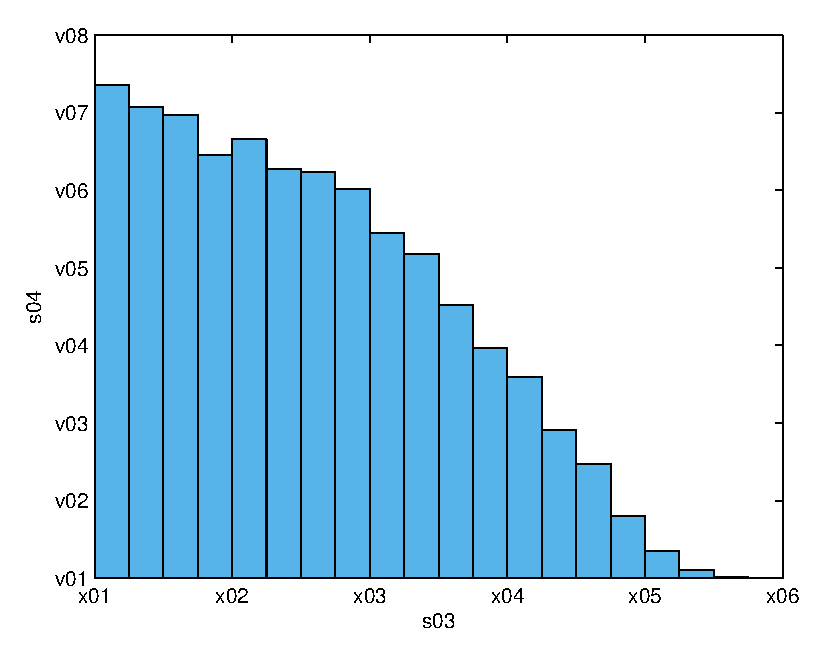
\includegraphics{Detect_SNR_hist.eps}}%
\end{psfrags}%
%
% End Detect_SNR_hist.tex
\end{document}
% See http://www.mathworks.de/matlabcentral/fileexchange/loadFile.do?objectId=4638
% for recent versions of laprint.m.
%
% created by:           LaPrint version 3.16 (13.9.2004)
% created on:           01-Nov-2013 11:27:56
% eps bounding box:     15 cm x 11.25 cm
% comment:              
%
\begin{psfrags}%
\psfragscanon%
%
% text strings:
\psfrag{s03}[t][t]{\color[rgb]{0,0,0}\setlength{\tabcolsep}{0pt}\begin{tabular}{c}{\Large$\rho$}\end{tabular}}%
\psfrag{s04}[b][b]{\color[rgb]{0,0,0}\setlength{\tabcolsep}{0pt}\begin{tabular}{c}{\Large Frequency per bin}\end{tabular}}%
%
% xticklabels:
\psfrag{x01}[t][t]{$10^1$}%
\psfrag{x02}[t][t]{$10^2$}%
\psfrag{x03}[t][t]{$10^3$}%
\psfrag{x04}[t][t]{$10^4$}%
\psfrag{x05}[t][t]{$10^5$}%
\psfrag{x06}[t][t]{$10^6$}%
\psfrag{x07}[t][t]{$10^7$}%
%
% yticklabels:
\psfrag{v01}[r][r]{$0$}%
\psfrag{v02}[r][r]{$500$}%
\psfrag{v03}[r][r]{$1000$}%
\psfrag{v04}[r][r]{$1500$}%
\psfrag{v05}[r][r]{$2000$}%
\psfrag{v06}[r][r]{$2500$}%
\psfrag{v07}[r][r]{$3000$}%
\psfrag{v08}[r][r]{$3500$}%
%
% Figure:
\resizebox{12cm}{!}{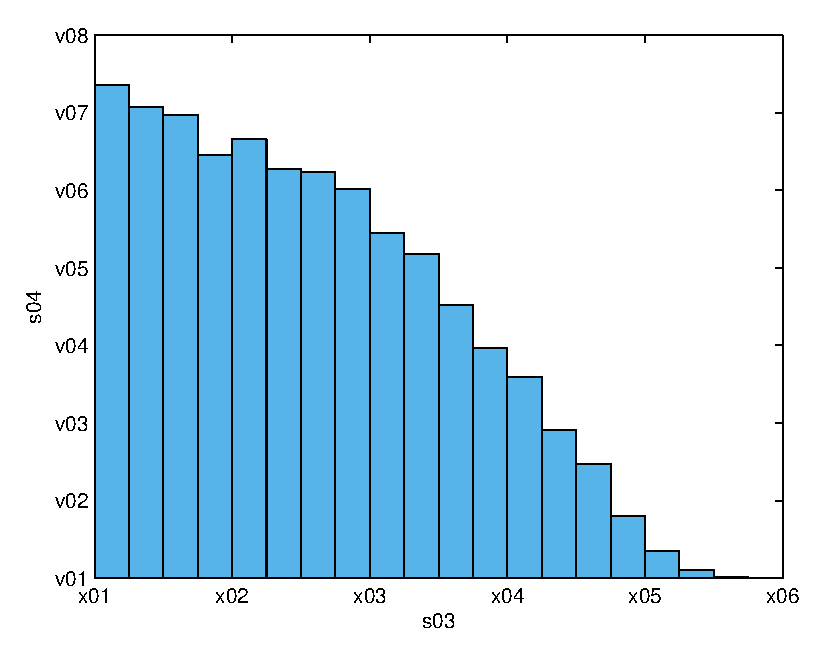
\includegraphics{Detect_SNR_hist.eps}}%
\end{psfrags}%
%
% End Detect_SNR_hist.tex
\end{document}
% See http://www.mathworks.de/matlabcentral/fileexchange/loadFile.do?objectId=4638
% for recent versions of laprint.m.
%
% created by:           LaPrint version 3.16 (13.9.2004)
% created on:           01-Nov-2013 11:27:56
% eps bounding box:     15 cm x 11.25 cm
% comment:              
%
\begin{psfrags}%
\psfragscanon%
%
% text strings:
\psfrag{s03}[t][t]{\color[rgb]{0,0,0}\setlength{\tabcolsep}{0pt}\begin{tabular}{c}{\Large$\rho$}\end{tabular}}%
\psfrag{s04}[b][b]{\color[rgb]{0,0,0}\setlength{\tabcolsep}{0pt}\begin{tabular}{c}{\Large Frequency per bin}\end{tabular}}%
%
% xticklabels:
\psfrag{x01}[t][t]{$10^1$}%
\psfrag{x02}[t][t]{$10^2$}%
\psfrag{x03}[t][t]{$10^3$}%
\psfrag{x04}[t][t]{$10^4$}%
\psfrag{x05}[t][t]{$10^5$}%
\psfrag{x06}[t][t]{$10^6$}%
\psfrag{x07}[t][t]{$10^7$}%
%
% yticklabels:
\psfrag{v01}[r][r]{$0$}%
\psfrag{v02}[r][r]{$500$}%
\psfrag{v03}[r][r]{$1000$}%
\psfrag{v04}[r][r]{$1500$}%
\psfrag{v05}[r][r]{$2000$}%
\psfrag{v06}[r][r]{$2500$}%
\psfrag{v07}[r][r]{$3000$}%
\psfrag{v08}[r][r]{$3500$}%
%
% Figure:
\resizebox{12cm}{!}{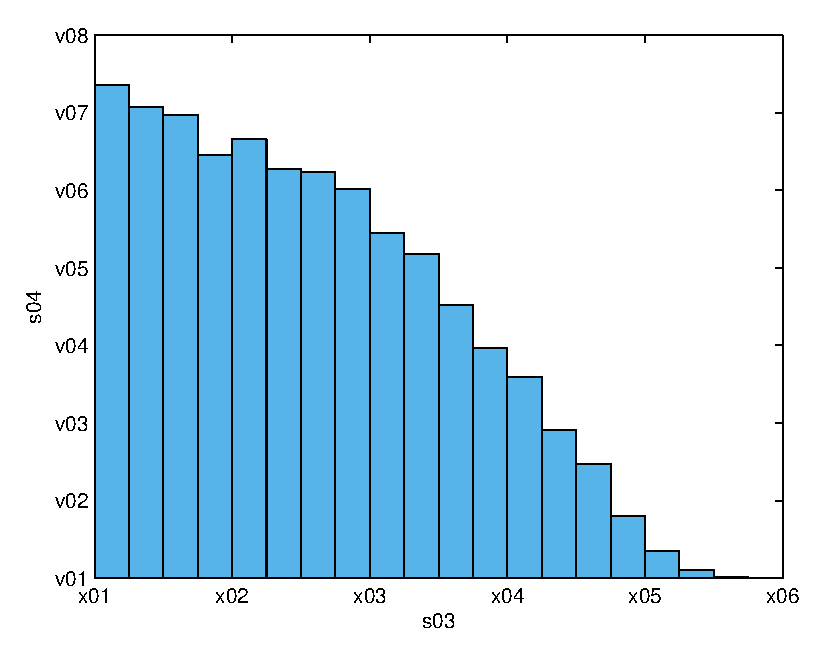
\includegraphics{Detect_SNR_hist.eps}}%
\end{psfrags}%
%
% End Detect_SNR_hist.tex
\end{document}
% See http://www.mathworks.de/matlabcentral/fileexchange/loadFile.do?objectId=4638
% for recent versions of laprint.m.
%
% created by:           LaPrint version 3.16 (13.9.2004)
% created on:           01-Nov-2013 11:27:56
% eps bounding box:     15 cm x 11.25 cm
% comment:              
%
\begin{psfrags}%
\psfragscanon%
%
% text strings:
\psfrag{s03}[t][t]{\color[rgb]{0,0,0}\setlength{\tabcolsep}{0pt}\begin{tabular}{c}{\Large$\rho$}\end{tabular}}%
\psfrag{s04}[b][b]{\color[rgb]{0,0,0}\setlength{\tabcolsep}{0pt}\begin{tabular}{c}{\Large Frequency per bin}\end{tabular}}%
%
% xticklabels:
\psfrag{x01}[t][t]{$10^1$}%
\psfrag{x02}[t][t]{$10^2$}%
\psfrag{x03}[t][t]{$10^3$}%
\psfrag{x04}[t][t]{$10^4$}%
\psfrag{x05}[t][t]{$10^5$}%
\psfrag{x06}[t][t]{$10^6$}%
\psfrag{x07}[t][t]{$10^7$}%
%
% yticklabels:
\psfrag{v01}[r][r]{$0$}%
\psfrag{v02}[r][r]{$500$}%
\psfrag{v03}[r][r]{$1000$}%
\psfrag{v04}[r][r]{$1500$}%
\psfrag{v05}[r][r]{$2000$}%
\psfrag{v06}[r][r]{$2500$}%
\psfrag{v07}[r][r]{$3000$}%
\psfrag{v08}[r][r]{$3500$}%
%
% Figure:
\resizebox{12cm}{!}{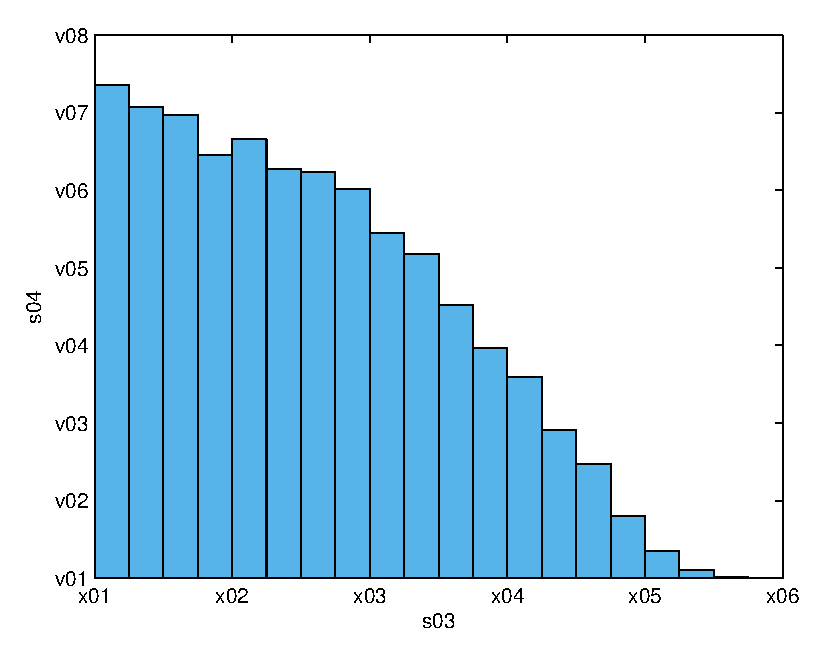
\includegraphics{Detect_SNR_hist.eps}}%
\end{psfrags}%
%
% End Detect_SNR_hist.tex
